\clearpage
%%=========================================
%\section[Surface Analysis of Substrate C with Surface Pre-Growth Preparation]{Surface Analysis of Substrate C with Surface Pre-Growth Preparation%
%    \sectionmark{Surface Analysis of Pre-Growth Substrate C}}\sectionmark{Surface Analysis of Pre-Growth Substrate C}\label{sec:subCb}

\section{Surface Analysis of Substrate C after Etching}
As substrate C was already polished by the vendor, the surface pre-growth preparation simply consisted of a \ce{Br}:methanol etch. The ultimate goal for the \ac{mbe} preparation etch was to provide a clean, smooth, and well-ordered surface to minimise growth defects. As can be seen in Fig.~\ref{fig:subCb_om_df}, there were many features larger than \SI{0.5}{\micro\metre} on the surface after the etch. The density of those features was \SI{\sim 8e3}{\centi\metre^{-1}}. 

\begin{figure}[htbp]
    \centering
    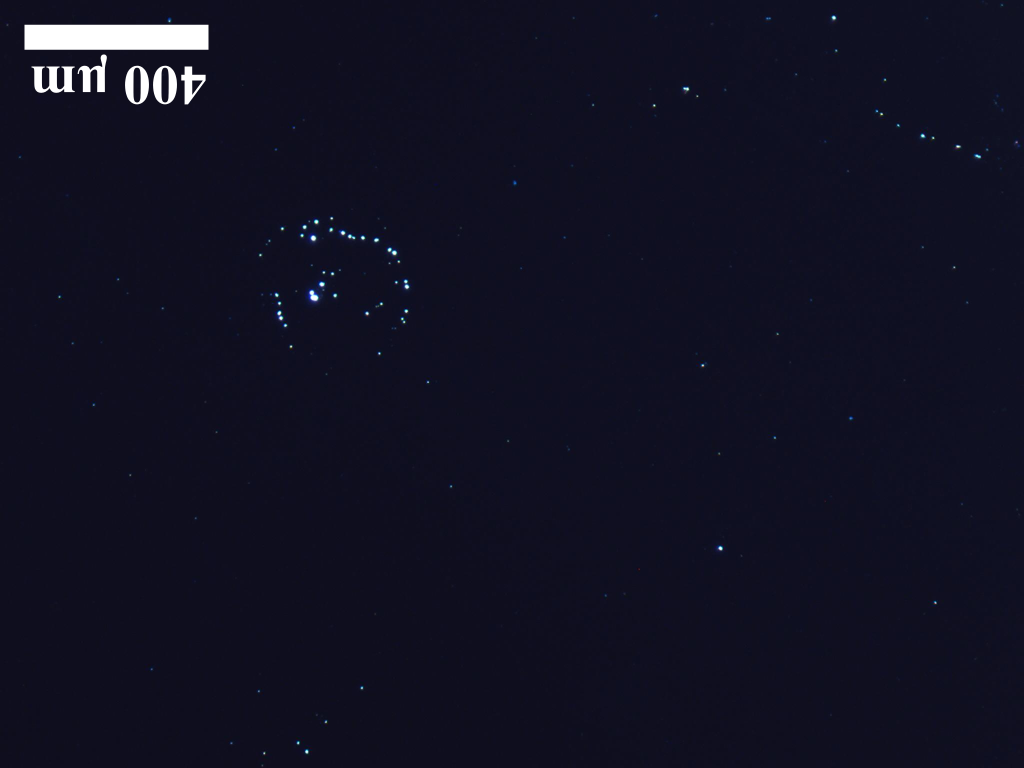
\includegraphics[width=0.8\linewidth, angle=180]{subCb_om_df_n018_5x.png}
    \caption[Dark field optical microscopy image of substrate C after \ce{Br}:methanol etch.]{Dark field optical microscopy image of substrate C after \ce{Br}:methanol etch taken near the centre of the substrate.}\label{fig:subCb_om_df}
\end{figure}

\Ac{sem} displayed the surface at a higher magnification and it revealed that there were smaller particles distributed over the surface as well. A typical area near the centre of the substrate can be seen in Fig.~\ref{fig:subCb_sem_typical_centre}. There were observed more particles close to the edge of the substrate, as seen in Fig.~\ref{fig:subCb_sem_typical_corner}. 

\begin{figure}[htbp]
    \mySubfigure{0.49\textwidth}{subCb_sem_04a_m008.png}[fig:subCb_sem_typical_centre]
    \hfill
    \mySubfigure{0.49\textwidth}{subCb_sem_04a_m005.png}[fig:subCb_sem_typical_corner]
    \caption[\Ac{sem} images of typical areas on substrate C with surface pre-growth preparation.]{\Ac{sem} images of \subref{fig:subCb_sem_typical_centre} a typical area near the centre and \subref{fig:subCb_sem_typical_corner} an area with a high density of particles near the edge of substrate C after surface pre-growth preparation.}\label{fig:subCb_sem_typical}
\end{figure}

%%=========================================
\subsection{Particles}

Four different types of particles were found and identified on the surface of the \ce{Br}:methanol etched substrate C, as seen in Fig.~\ref{fig:subCb_sem_w_eds}.

\begin{figure}[htbp]
    \centering
    \begin{subfigure}[t]{\textwidth}
        \caption{}\label{fig:subCb_silica}
          \begin{minipage}[c]{0.43\linewidth}
            \centering
            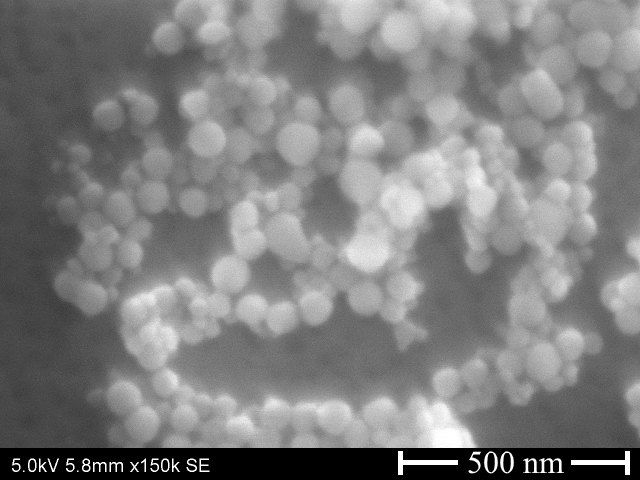
\includegraphics[width=\linewidth]{subCb_sem_07_m002.png}
          \end{minipage}
          \hfill
          \begin{minipage}[c]{0.43\linewidth}
            \centering
            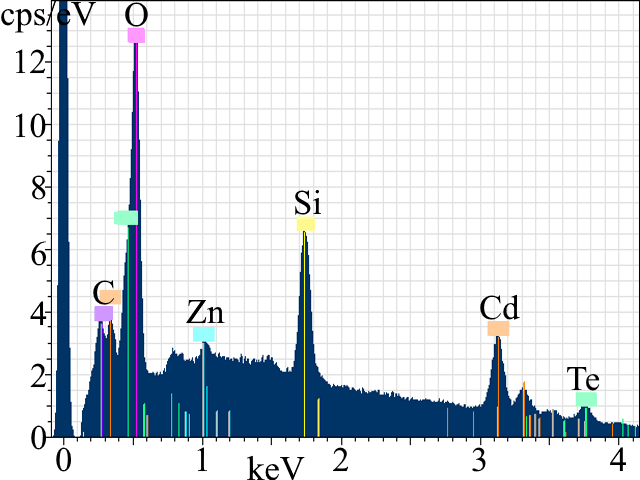
\includegraphics[width=\linewidth]{subCb_sem_07_m002_eds.png}
          \end{minipage}
          \begin{minipage}[c]{0.11\linewidth}
            \centering
            \atomicTable[\ce{O}&\SI{41.32}{}][\ce{Si}&\SI{33.82}{}][\ce{Cd}&\SI{10.63}{}][\ce{Te}&\SI{10.17}{}][\ce{C}&\SI{3.22}{}][\ce{Zn}&\SI{0.59}{}][\ce{Al}&\SI{0.25}{}]
          \end{minipage}
    \end{subfigure}
    \par\bigskip
    \begin{subfigure}[t]{\textwidth}
        \caption{}\label{fig:subCb_silica_large}
          \begin{minipage}[c]{0.43\linewidth}
            \centering
            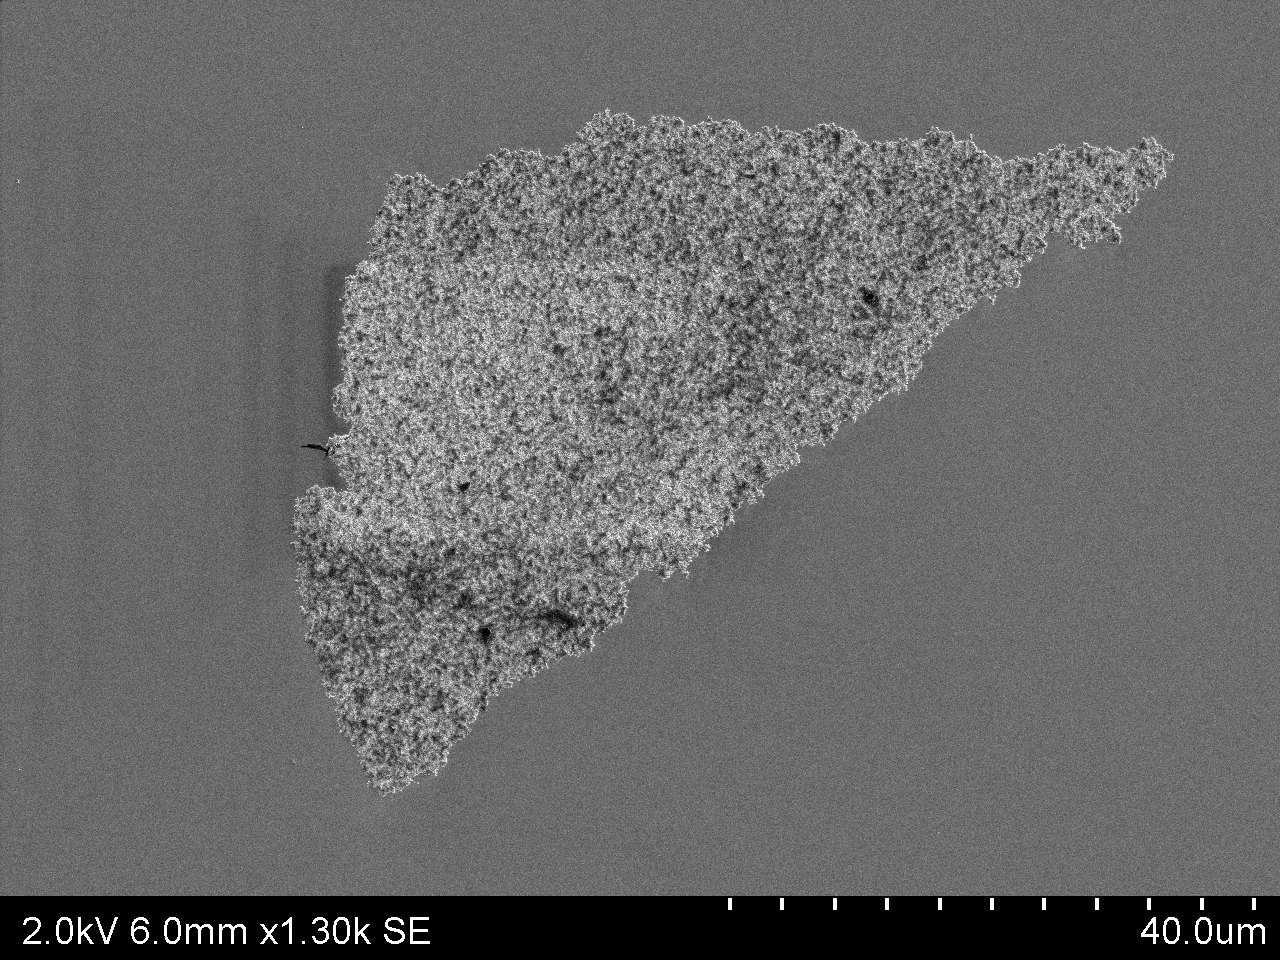
\includegraphics[width=\linewidth]{subCb_sem_03_m010.png}
          \end{minipage}
          \hfill
          \begin{minipage}[c]{0.43\linewidth}
            \centering
            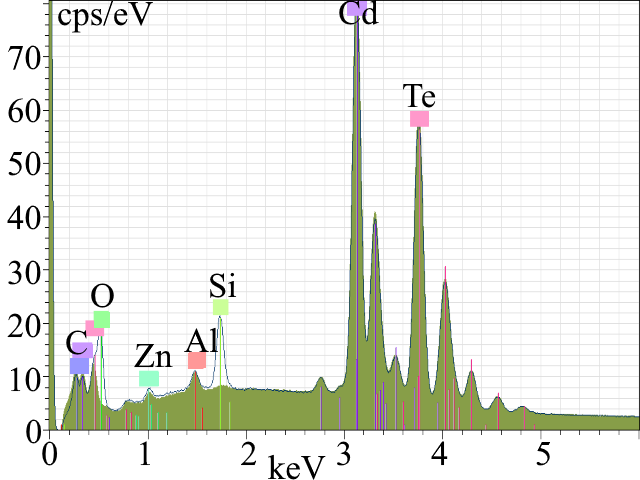
\includegraphics[width=\linewidth]{subCb_sem_03_m010_eds.png}
          \end{minipage}
          \begin{minipage}[c]{0.11\linewidth}
            \centering
            \atomicTable[\ce{Cd}&\SI{34.46}{}][\ce{Te}&\SI{34.30}{}][\ce{O}&\SI{16.82}{}][\ce{Si}&\SI{7.51}{}][\ce{C}&\SI{3.90}{}][\ce{Al}&\SI{1.66}{}][\ce{Zn}&\SI{1.25}{}]
          \end{minipage}
    \end{subfigure}
    \begin{subfigure}[t]{\textwidth}
        \caption{}\label{fig:subCb_Br-etch}
          \begin{minipage}[c]{0.43\linewidth}
            \centering
            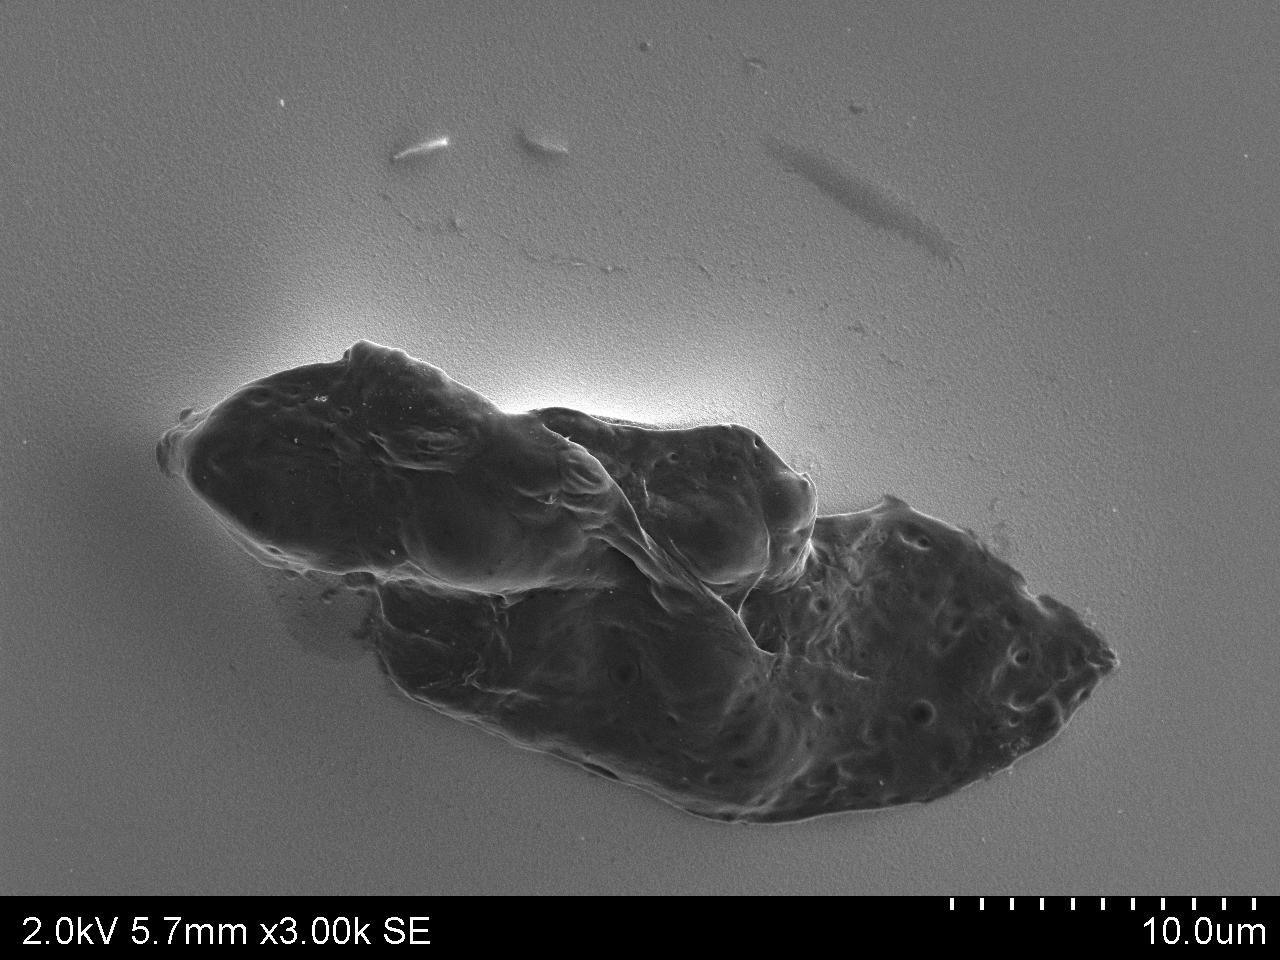
\includegraphics[width=\linewidth]{subCb_sem_03_m001.png}
          \end{minipage}
          \hfill
          \begin{minipage}[c]{0.43\linewidth}
            \centering
            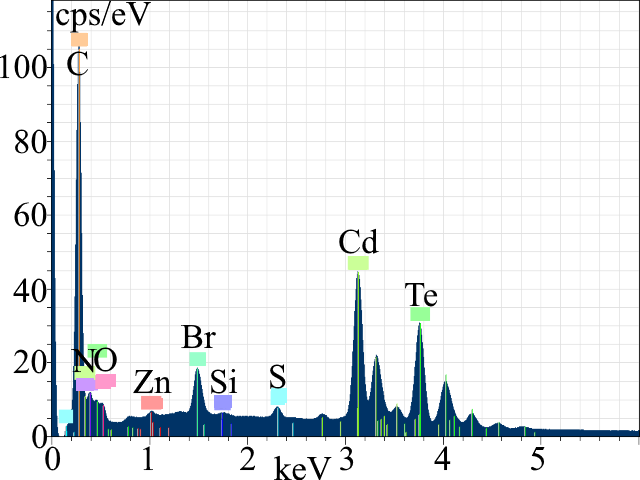
\includegraphics[width=\linewidth]{subCb_sem_03_m001_eds.png}
          \end{minipage}
          \begin{minipage}[c]{0.11\linewidth}
            \centering
            \atomicTable[\ce{C}&\SI{60.68}{}][\ce{Cd}&\SI{12.24}{}][\ce{Te}&\SI{11.78}{}][\ce{N}&\SI{8.31}{}][\ce{O}&\SI{3.97}{}][\ce{Br}&\SI{2.20}{}][\ce{S}&\SI{0.82}{}]
          \end{minipage}
    \end{subfigure}
    \par\bigskip
    \caption[\Ac{sem} images, \ac{eds} spectra, and \ac{eds} atomic compositions of two different types of particles found on substrate C after surface pre-growth preparation.]{High resolution \ac{sem} images of two different types of particles found on substrate C after surface pre-growth preparation and the corresponding \ac{eds} spectra and atomic compositions: \subref{fig:subCb_silica} Silica (\ce{SiO2}) polishing grit; \subref{fig:subCb_silica_large} large silica agglomeration; and \subref{fig:subCb_Br-etch}--\subref{fig:subCb_Br-etch2} carbon-based particles.}\label{fig:subCb_sem_w_eds}
\end{figure}
%
\begin{figure}[htbp]
\ContinuedFloat
    \centering
    \begin{subfigure}[t]{\textwidth}
        \caption{}\label{fig:subCb_Br-etch2}
          \begin{minipage}[c]{0.43\linewidth}
            \centering
            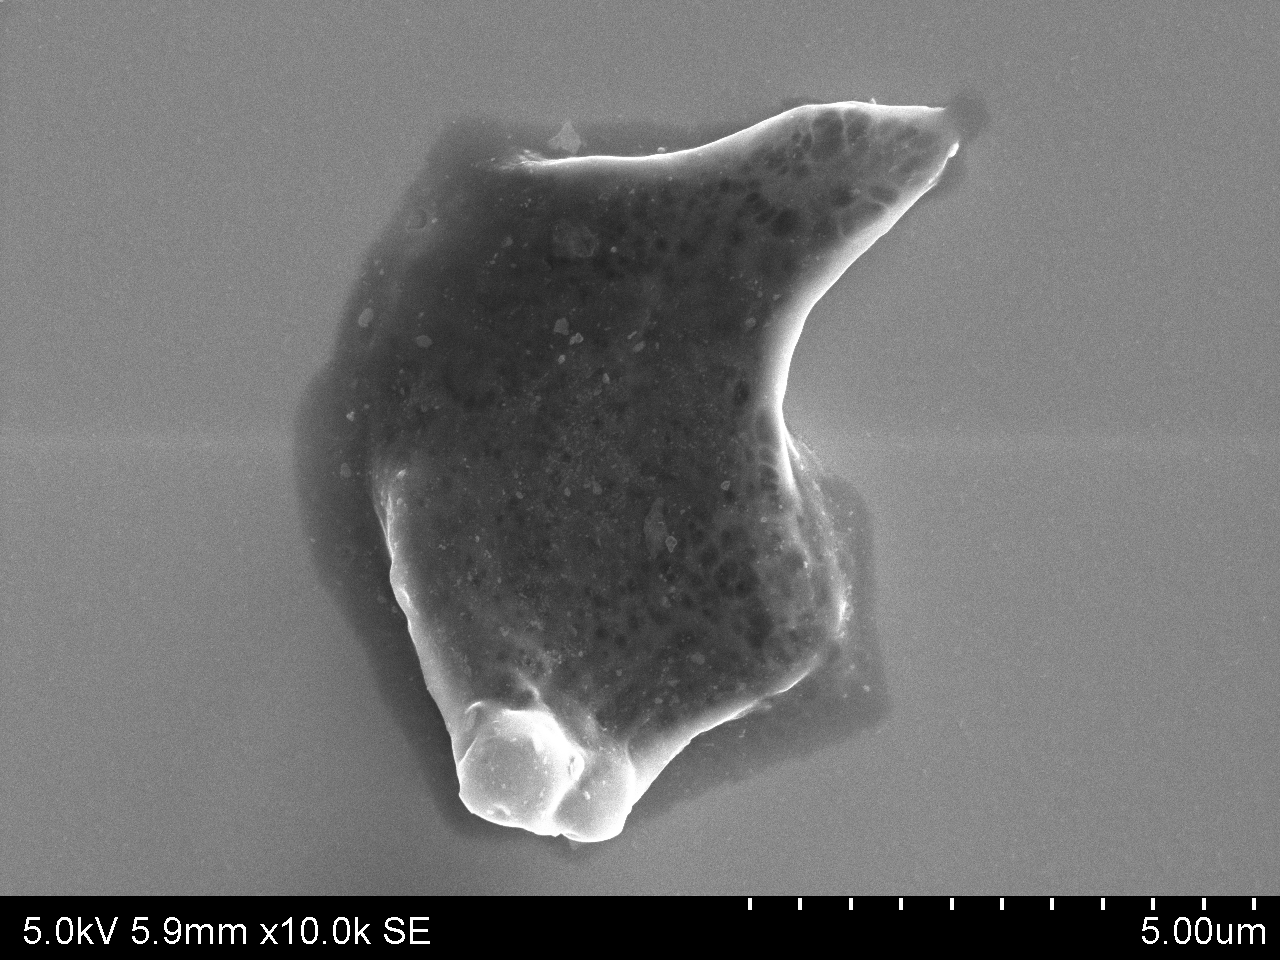
\includegraphics[width=\linewidth]{subCb_sem_09_m004.png}
          \end{minipage}
          \hfill
          \begin{minipage}[c]{0.43\linewidth}
            \centering
            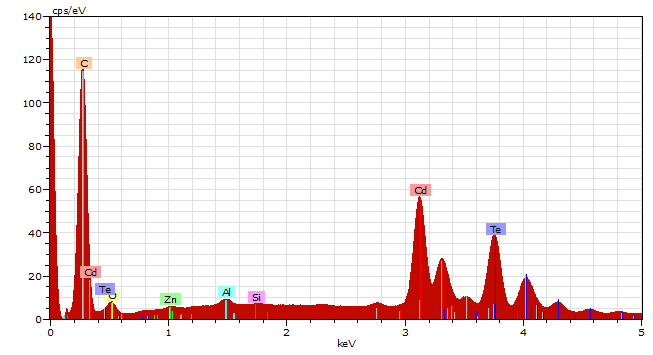
\includegraphics[width=\linewidth]{subCb_sem_09_m004_eds.png}
          \end{minipage}
          \begin{minipage}[c]{0.11\linewidth}
            \centering
            \atomicTable[\ce{C}&\SI{66.58}{}][\ce{Cd}&\SI{14.56}{}][\ce{Te}&\SI{13.80}{}][\ce{O}&\SI{4.02}{}][\ce{Br}&\SI{0.55}{}][\ce{Zn}&\SI{0.48}{}]
          \end{minipage}
    \end{subfigure}
    \captionsetup{list=no}
    \caption{\emph{(continued)}}
\end{figure}

\subsubsection{Silica (\ce{SiO2}) polishing grit and agglomerations}

Silica polishing grit were found on the surface of the substrate after \ce{Br}:methanol etch, see Fig.~\ref{fig:subCb_silica}. However, the polishing grit density was lower than before the etch. The silica polishing grit were found all over the surface with a tendency of higher density towards the upper right, lower right, and lower left corners. The particle density was found to be between \SI{2e+05}{\centi\metre^{-2}} and \SI{1e+07}{\centi\metre^{-2}}. The average particle density was \SI{3e+06}{\centi\metre^{-2}}, with a standard deviation of \SI{3e+06}{\centi\metre^{-2}}. The polishing grit density was reduced by a factor 10 compared to the average density before etch. A graphical representation of the particle density at 25 different locations on substrate C can be seen in Fig.~\ref{fig:subCb_densityData}. The sample Pearson correlation coefficient demonstrated that there was a weak negative correlation of \SI{-0.3}{} between the density of polishing grit on the as-received substrate C and the density of polishing grit after surface pre-growth preparation. This was not enough to claim that the density before and after preparation was correlated.

Some large silica agglomerations with size ranging up to \SI{50}{\micro\metre} were observed near the edges of substrate C, see Fig.~\ref{fig:subCb_silica_large}. As the \ac{eds} spectrum had \ac{czt} as the major contributor to the signal, this indicates that the grit particles form a thin layer on the surface. The silica particles from the as-received substrate could have been redistributed over the surface by the etch solution and at the same time collected into larger agglomerations.

\begin{figure}[htbp]
    \centering
    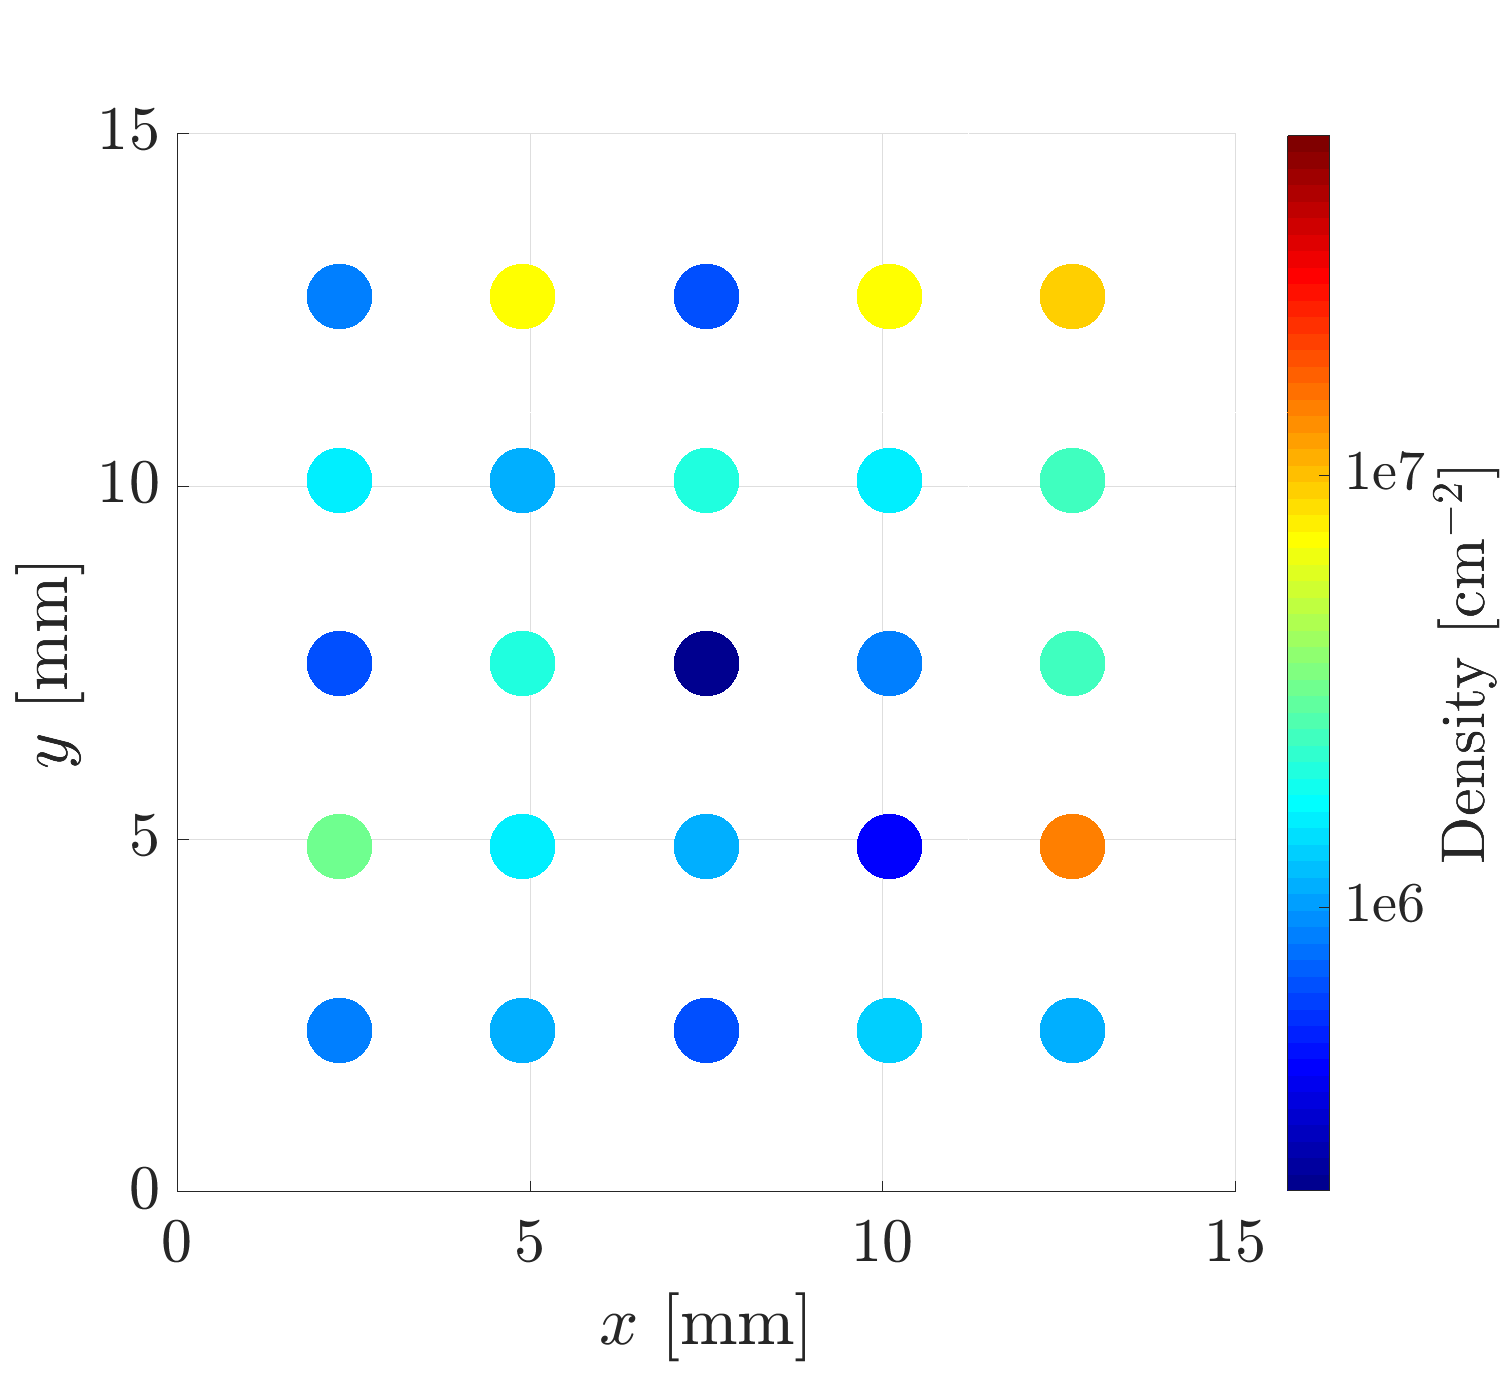
\includegraphics[width=0.5\linewidth]{subCb_densityData.png}
    \caption[Map of the polishing grit density on substrate C after surface pre-growth preparation.]{A map of the polishing grit density at 25 different locations on the $\SI{15}{\milli\metre}\times\SI{15}{\milli\metre}$ substrate C after surface pre-growth preparation. The density measurements were obtained by counting the number of polishing grits in \ac{sem} images covering $\SI{25.4}{\micro\metre}\times\SI{17.8}{\micro\metre}$ areas. In total, \SI{0.005}{\percent} of the substrate surface was measured. The polishing grit density was observed to vary between \SI{2e+05}{\centi\metre^{-2}} and \SI{1e+07}{\centi\metre^{-2}}.}
    \label{fig:subCb_densityData}
\end{figure}

\subsubsection{Carbon-based particles}
In addition to the polishing grit, some larger particles with size \SIrange{5}{10}{\micro\metre} was observed on the surface, as seen in Fig.~\ref{fig:subCb_Br-etch} and Fig.~\ref{fig:subCb_Br-etch2}. The particles consisted mainly of carbon and could be the same carbon-based particles from before the etch. The signal from nitrogen was also present before etch, but the bromine would come from the \ce{Br}:methanol etch and had possibly sticked to the carbon-based particle.


%%=========================================
%\section{AFM Study of Etched Substrate C}
\subsection{Surface Roughness}

The \ce{Br}:methanol etched substrate C was characterised for surface topography by \ac{afm}. Images of $\SI{5}{\micro\metre}\times\SI{5}{\micro\metre}$ areas were taken at three different locations on the substrate surface: near the centre, upper edge, and upper left corner, as seen in Fig.~\ref{fig:subCb_afm}. The \ac{rms} roughness was calculated to be \SI{1.4}{\nano\metre}, \SI{1.4}{\nano\metre}, and \SI{2.8}{\nano\metre}, respectively, using Eq.~\ref{eq:rmsroughness}. The roughness had increased by \SI{50}{\percent} near the centre, indifferent at the edge, and increased by a factor 2 near the corner compared to the substrate before etch.

\begin{figure}[htbp]
    \centering
    \begin{subfigure}[c]{0.032\linewidth}
        \label{fig:subCb_afm_scale}\captionsetup{list=no}
        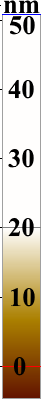
\includegraphics[width=\linewidth]{subCb_afm_scale.png}
    \end{subfigure}
    \hfill
    \mySubfigure{0.3\linewidth}{subCb_afm_centre.png}[fig:subCb_afm_centre]  %\SI{0.85}{\nano\metre}}
    \hfill
    \mySubfigure{0.3\linewidth}{subCb_afm_upperedge.png}[fig:subCb_afm_edge]  %\SI{0.77}{\nano\metre}}
    \hfill
    \mySubfigure{0.3\linewidth}{subCb_afm_upperleftcorner.png}[fig:subCb_afm_corner]  %\SI{1,04}{\nano\metre}}
    \caption[\Ac{afm} of substrate C with surface pre-growth preparation.]{\Ac{afm} measurements of substrate C with surface pre-growth preparation. Images of $\SI{5}{\micro\metre}\times\SI{5}{\micro\metre}$ areas are taken at three different locations on the substrate surface: \subref{fig:subCb_afm_centre} near the centre, \ac{rms} roughness \SI{1.4}{\nano\metre}; \subref{fig:subCb_afm_edge} near the upper edge, \ac{rms} roughness \SI{1.4}{\nano\metre}; and \subref{fig:subCb_afm_corner} near the upper left corner, \ac{rms} roughness \SI{2.8}{\nano\metre}.}
    \label{fig:subCb_afm}
\end{figure} % AFM, substrate C, with surface pre-growth preparation.

%%=========================================
\subsection{Impurity Analysis -- EDS}

\Ac{eds} was used to get a quantitative analysis of the chemical composition of substrate C after a \ce{Br}:methanol etch. The results can be seen in Table~\ref{tab:subCb_eds_analysis}. The same elements were identified as before the etch: \ce{Te}, \ce{Cd}, \ce{Zn}, \ce{Al}, \ce{Si}, \ce{C}, and \ce{O}. The atomic concentration of \ce{Si} was the same as before the etch, which was surprising as the polishing grit density was reduced by a factor of 10. 

\begin{table}[htbp]
    \centering
    \caption[\Ac{eds} impurity analysis of substrate C with surface pre-growth preparation.]{Results of the \ac{eds} impurity analysis at three different locations on the $\SI{15}{\milli\metre}\times\SI{15}{\milli\metre}$ (211)B \ac{czt} substrate C with surface pre-growth preparation (atomic concentration \%). The X-ray signal was acquired from $\SI{1270}{\micro\metre}\times\SI{890}{\micro\metre}$ areas near the centre, upper edge, and upper left corner.}\label{tab:subCb_eds_analysis}
    \begin{tabu} to 1.0\textwidth { X[1.85,r] X[1.125,c] X[1.125,c] X[1.125,c] X[1.125,c] X[1.125,c] X[1.125,c] X[1.125,c] }
    \hline
         & \textbf{\ce{Te}} (at.\%) & \textbf{\ce{Cd}} (at.\%) & \textbf{\ce{Zn}} (at.\%) & \textbf{\ce{Al} } (at.\%) & \textbf{\ce{Si}} (at.\%) & \textbf{\ce{C}} (at.\%) & \textbf{\ce{O}} (at.\%) \\
        \hline
        Near centre & \SI{44.70}{} & \SI{44.56}{} & \SI{1.43}{} & \SI{2.12}{} & \SI{0.51}{} & \SI{5.78}{} & \SI{0.90}{} \\
        Near edge   & \SI{44.31}{} & \SI{44.38}{} & \SI{1.42}{} & \SI{2.31}{} & \SI{0.53}{} & \SI{6.01}{} & \SI{1.05}{} \\ 
         Near corner & \SI{44.67}{} & \SI{44.77}{} & \SI{1.38}{} & \SI{1.77}{} & \SI{0.53}{} & \SI{5.79}{} & \SI{1.10}{} \\ 
         \hline
    \end{tabu}
\end{table}

%%=========================================